\section*{Тестирование программы}

Запустим программу введём случайное слово. 
Программа не распознает комманду и предложит 
использовать 'help' (рис.\ref{test.unknown_command}). 

\begin{figure}[hpt!]
    \centering
    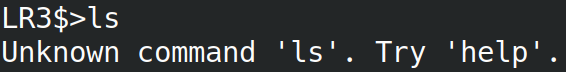
\includegraphics[width=0.9\linewidth]{photo/test.unknown_command}
    \caption{Неизвестная команда}
    \label{test.unknown_command}
\end{figure}

Введём команду 'help', чтобы получить справку (рис. \ref{test.help}).

\begin{figure}[hpt!]
    \centering
    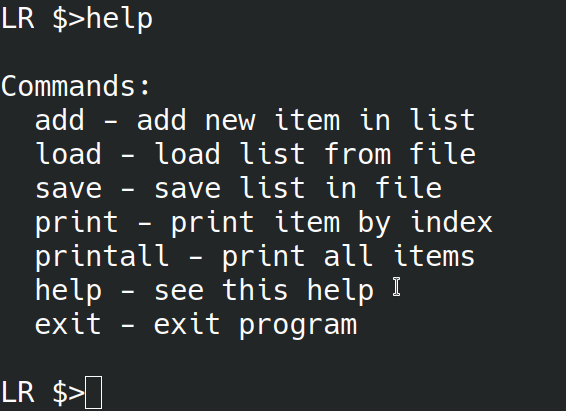
\includegraphics[width=0.9\linewidth]{photo/test.help}
    \caption{Справка}
    \label{test.help}
\end{figure}

На попытки распечатать элементы пустого списка
программа отвечает, что нечего печатать и предлагает
использовать команду 'add' (рис. \ref{test.print_empty}).

\begin{figure}[H]
    \centering
    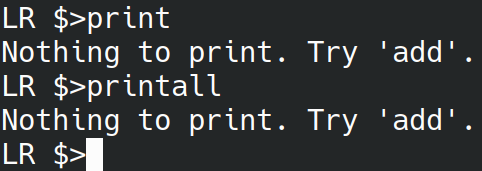
\includegraphics[width=0.9\linewidth]{photo/test.print_empty}
    \caption{Печть пустого списка}
    \label{test.print_empty}
\end{figure}

Добавим 2 элемента в список, используя 'add'(рис.\ref{test.add}, \ref{test.add2}).
В случае попытки ввести некорректные данные 
ввод зацикливается (рис.\ref{test.add}) до тех пор,
пока не будут введены корректные данные.

\begin{figure}[H]
    \centering
    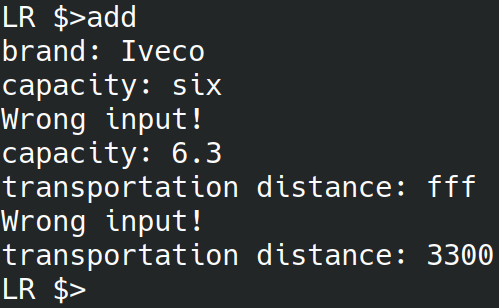
\includegraphics[width=0.9\linewidth]{photo/test.add}
    \caption{Добавление 1 элемента в список}
    \label{test.add}
\end{figure}

\begin{figure}[H]
    \centering
    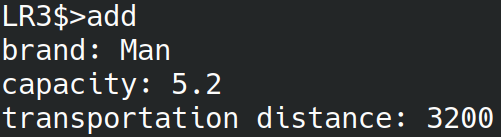
\includegraphics[width=0.9\linewidth]{photo/test.add2}
    \caption{Добавление 2 элемента в список}
    \label{test.add2}
\end{figure}

Распечатаем первый элемент (с индексом 0) с помощью команды 'print' (рис.\ref{test.print0}).

\begin{figure}[hpt!]
    \centering
    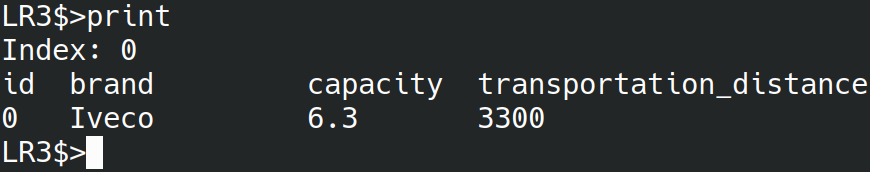
\includegraphics[width=0.9\linewidth]{photo/test.print0}
    \caption{Вывод первого элемента}
    \label{test.print0}
\end{figure}

Распечатаем все элементы списка с помощью команды 'printall' (рис.\ref{test.printall}).

\begin{figure}[hpt!]
    \centering
    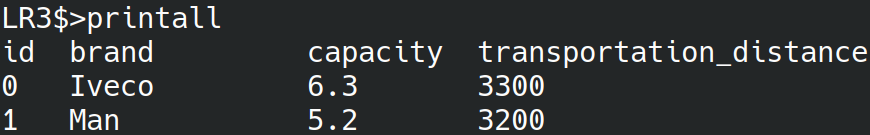
\includegraphics[width=0.9\linewidth]{photo/test.printall}
    \caption{Вывод элементов списка}
    \label{test.printall}
\end{figure}

Сохраним текущий список.

Если попытаться передать директорию, программа не сохранит файл (рис. \ref{test.save.dir}). 

\begin{figure}[hpt!]
    \centering
    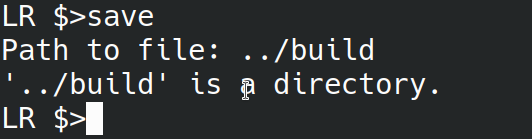
\includegraphics[width=0.9\linewidth]{photo/test.save.dir}
    \caption{Сохранение файла под именем директории}
    \label{test.save.dir}
\end{figure}

Если попытаться перезаписать существующий файл, программа попросит подтверждение.

Можно отказаться (рис. \ref{test.save.n}).

\begin{figure}[hpt!]
    \centering
    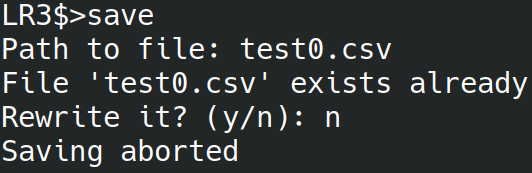
\includegraphics[width=0.9\linewidth]{photo/test.save.n}
    \caption{Отказ от перезаписи}
    \label{test.save.n}
\end{figure}

Можно согласиться (рис. \ref{test.save.y}).

\begin{figure}[hpt!]
    \centering
    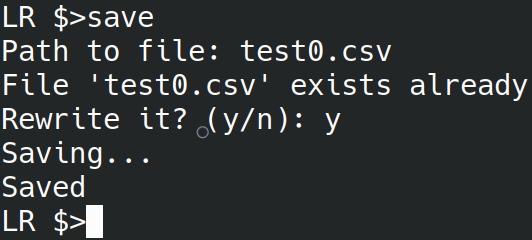
\includegraphics[width=0.9\linewidth]{photo/test.save.y}
    \caption{Соглашение на перезапись}
    \label{test.save.y}
\end{figure}

Сохранённый файл виден на рис. \ref{test.file}.

\begin{figure}[hpt!]
    \centering
    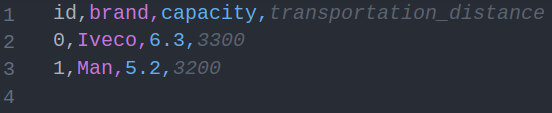
\includegraphics[width=0.9\linewidth]{photo/test.file}
    \caption{Сохранённый файл}
    \label{test.file}
\end{figure}

При загрузке файла программа выдаст предупреждение, что 
загрузка перезапишет текущий список, и попросит подтверждение (рис. \ref{test.load.exist})

\begin{figure}[hpt!]
    \centering
    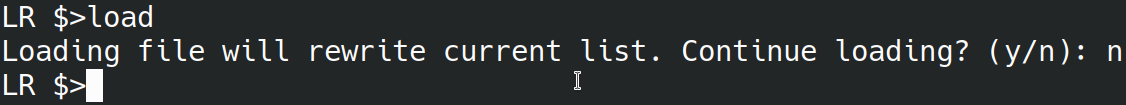
\includegraphics[width=0.9\linewidth]{photo/test.load.exist}
    \caption{Предупреждение при загрузке файла}
    \label{test.load.exist}
\end{figure}

Перезапустим программу, чтобы очистить список.

Попытаемся загрузить файл (рис.\ref{test.file}) с помощью команды 'load'.

При попытке передачи директории или несуществующего файла, 
программа предупредит об этом и остановит загрузку.
Загрузим файл и проверим, что данные считались корректно 
с помощью команды 'printall' (рис.\ref{test.load}).

\begin{figure}[hpt!]
    \centering
    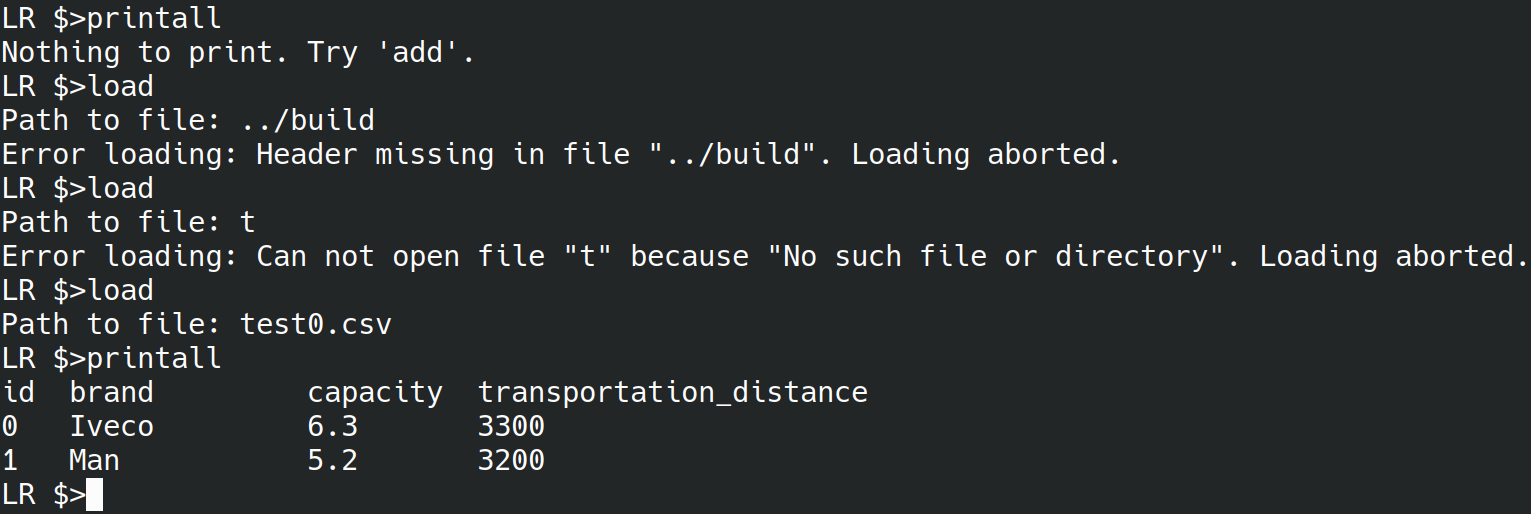
\includegraphics[width=0.9\linewidth]{photo/test.load}
    \caption{Загрузка файла}
    \label{test.load}
\end{figure}